\documentclass{article}
\usepackage[utf8]{inputenc}
\usepackage{amsmath}
\usepackage{graphicx}
\usepackage{float}
\title{Analysis Report on Publibike Dataset}
%\author{howard.hao.ma }
%\date{November 2019}

\begin{document}

\maketitle
\newpage
\section{Data Description:} 
We merged the following data:
\begin{itemize}
    \item Publibike: total number of Publibike rides by hour
    \item Swisscom: total number of Swisscom commuters in Lugano by hour
    \item TPL: total number of total running buses by hour
\end{itemize}
\newpage

\section{Substitution Effect btw Buses and Publibikes }
\subsection{All Sample}
\begin{align}
    y_i  = \beta_1 + \beta_2 x_i + \varepsilon_i, \label{model1}
\end{align}
where $y_i$ represents the number of rides per hour, and $x_i$ represents the number of Swisscom commuters per hour.\\

% Table created by stargazer v.5.2.2 by Marek Hlavac, Harvard University. E-mail: hlavac at fas.harvard.edu
% Date and time: Sat, Nov 16, 2019 - 23:03:52
\begin{table}[H]\centering 
  \caption{All sample} 
  \label{} 
\begin{tabular}{@{\extracolsep{5pt}}lc} 
\\[-1.8ex]\hline 
\hline \\[-1.8ex] 
 & \multicolumn{1}{c}{\textit{Dependent variable:}} \\ 
\cline{2-2} 
\\[-1.8ex] & \# rides per hour\\ 
\# Swisscom commuters per hour & 0.005$^{***}$ \\ 
  & (0.001) \\ 
  & \\ 
 Constant & 24.172$^{***}$ \\ 
  & (1.070) \\ 
  & \\ 
\hline \\[-1.8ex] 
Observations & 768 \\ 
R$^{2}$ & 0.072 \\ 
Adjusted R$^{2}$ & 0.071 \\ 
Residual Std. Error & 18.833 (df = 766) \\ 
F Statistic & 59.793$^{***}$ (df = 1; 766) \\ 
\hline 
\hline \\[-1.8ex] 
\textit{Note:}  & \multicolumn{1}{r}{$^{*}$p$<$0.1; $^{**}$p$<$0.05; $^{***}$p$<$0.01} \\ 
\end{tabular} 
\end{table} 

\subsection{By bus coverage}
\begin{figure}[H]
    \centering
    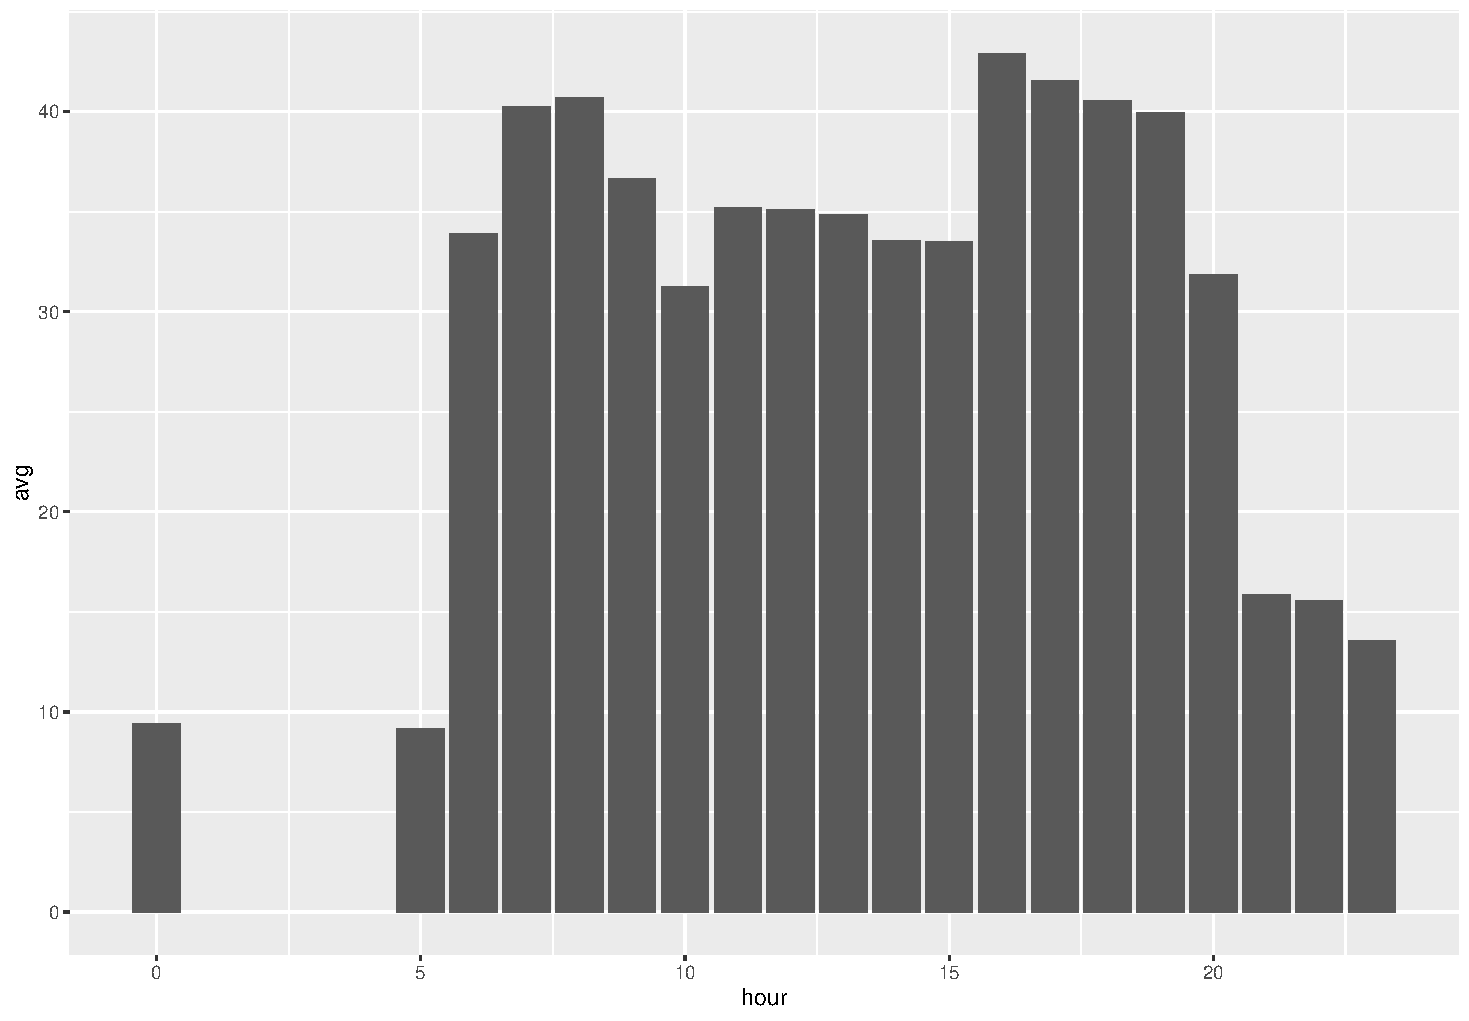
\includegraphics[width = \textwidth]{tpl_density.pdf}
    \caption{Histogram of number of running buses by hour}
    \label{fig:my_label}
\end{figure}

\begin{align}
    y_i(S)  = \beta_1 + \beta_2 x_i (S) I_D + \varepsilon_i 
\end{align}
where $S = D, E, N$. 
\begin{itemize}
    \item $D:$ day time 6am-8pm, enough buses on the road
    \item $E:$ evening time 9pm-0am and 5am, a few buses on the road
    \item $N:$ night time 1am-4am, no buses on the road
\end{itemize}

% Table created by stargazer v.5.2.2 by Marek Hlavac, Harvard University. E-mail: hlavac at fas.harvard.edu
% Date and time: Sat, Nov 16, 2019 - 23:03:53
\begin{table}[H] \centering 
  \caption{Subsititution effect by bus coverage} 
  \label{} 
\begin{tabular}{@{\extracolsep{5pt}}lccc} 
\\[-1.8ex]\hline 
\hline \\[-1.8ex] 
 & \multicolumn{3}{c}{\textit{Dependent variable:} \# Publibike rides per hour}\\ 
\cline{2-4} 
\\[-1.8ex] & 6am - 8pm & 9pm - 0am and 5am & 1am - 4am\\ 
\hline \\[-1.8ex] 
 \# Swisscom commuters & 0.003$^{***}$ & 0.088$^{***}$ & 0.113$^{**}$ \\ 
  & (0.001) & (0.013) & (0.043) \\ 
  & & & \\ 
 Constant & 28.600$^{***}$ & 7.525$^{**}$ & 3.666$^{*}$ \\ 
  & (1.657) & (3.729) & (2.150) \\ 
  & & & \\ 
\hline \\[-1.8ex] 
Observations & 521 & 174 & 73 \\ 
R$^{2}$ & 0.022 & 0.212 & 0.089 \\ 
Adjusted R$^{2}$ & 0.020 & 0.207 & 0.076 \\ 
Residual Std. Error & 16.594 (df = 519) & 21.521 (df = 172) & 8.434 (df = 71) \\ 
F Statistic & 11.759$^{***}$ (df = 1; 519) & 46.293$^{***}$ (df = 1; 172) & 6.902$^{**}$ (df = 1; 71) \\ 
\hline 
\hline \\[-1.8ex] 
\textit{Note:}  & \multicolumn{3}{r}{$^{*}$p$<$0.1; $^{**}$p$<$0.05; $^{***}$p$<$0.01} \\ 
\end{tabular} 
\end{table} 

\subsection{Conclusions and suggestions}
\begin{enumerate}
    \item A lower ratio of commuters will use Publibikes when there are more buses available
    \item From 9pm to 4am, around 10\% of commuters use Publibikes, which is way higher than day time, 0.3\%
    \item During the evening time, the R square of the model reaches 21.2\%, which means 20\% of the changes in demands for Publibikes are driven by commuters.
    \item Publibike company should consider pushing ads designed for commuters  during evening time. (Precise marketing)
\end{enumerate}

\newpage

\section{User Type Impact on the Usage of Publibike}
\textbf{Causality Issue: } Both the usage of Publibikes and buses will be driven by the commuting demands during peak hours. We need to control for that by gathering the residuals first:
\begin{align}
    e_i^y = y_i - \hat{\beta}_1 + \hat{\beta}_2 z_i\\
    e_i^x = x_i - \hat{\gamma}_1 + \hat{\gamma}_2 z_i
\end{align}
where $z_i$ is the number of buses that are on the road. Then we run the following regression:
\begin{align}
    e_i^y(T) = \theta_0 + \theta_1 e_i^x(T) + \varepsilon_i,
\end{align}
where $T =$ 'summer' or 'not summer'.


% Table created by stargazer v.5.2.2 by Marek Hlavac, Harvard University. E-mail: hlavac at fas.harvard.edu
% Date and time: Sun, Nov 17, 2019 - 10:46:58
\begin{table}[!htbp] \centering 
  \caption{} 
  \label{} 
\begin{tabular}{@{\extracolsep{5pt}}lcc} 
\\[-1.8ex]\hline 
\hline \\[-1.8ex] 
 & \multicolumn{2}{c}{\textit{Dependent variable:}} \\ 
\cline{2-3} 
\\[-1.8ex] & \multicolumn{2}{c}{Residuals of (\# number of Publibike rides)} \\ 
\\[-1.8ex] & Before summer holiday & Summer holiday\\ 
\hline \\[-1.8ex] 
 Residuals of \\
 (\# number of Swisscom commuters) & 0.003$^{**}$ & 0.0005 \\ 
  & (0.001) & (0.002) \\ 
  & & \\ 
 Constant & $-$0.000 & $-$0.000 \\ 
  & (0.923) & (1.062) \\ 
  & & \\ 
\hline \\[-1.8ex] 
Observations & 237 & 284 \\ 
R$^{2}$ & 0.028 & 0.0003 \\ 
Adjusted R$^{2}$ & 0.024 & $-$0.003 \\ 
Residual Std. Error & 14.216 (df = 235) & 17.890 (df = 282) \\ 
F Statistic & 6.711$^{**}$ (df = 1; 235) & 0.094 (df = 1; 282) \\ 
\hline 
\hline \\[-1.8ex] 
\textit{Note:}  & \multicolumn{2}{r}{$^{*}$p$<$0.1; $^{**}$p$<$0.05; $^{***}$p$<$0.01} \\ 
\end{tabular} 
\end{table} 

\subsection{Conclusions and suggestions}
\begin{enumerate}
    \item Students are the major users of Publibikes
    \item Employees don't ride Publibikes more often even if there are more bikes available during the summer holiday.
    \item To promote sustainability, employers should encourage employees use Publibikes more often especially during the summer holiday.
\end{enumerate}

\end{document}
